\section{設計}
        今回測定したサンプルは3つである。作成時期順に列挙すると、基本形となるrf-SQUIDを共振器間に配置したLCC。そしてrf-SQUIDと共振器間の結合部にジョセフソン接合を導入したJLCC、最後に接合部をミアンダインダクタンスに変更したMLCCである。まずは基本型の構造は先行論文がとっている手法と全く同じである。
        \begin{figure}[H]
            \centering
            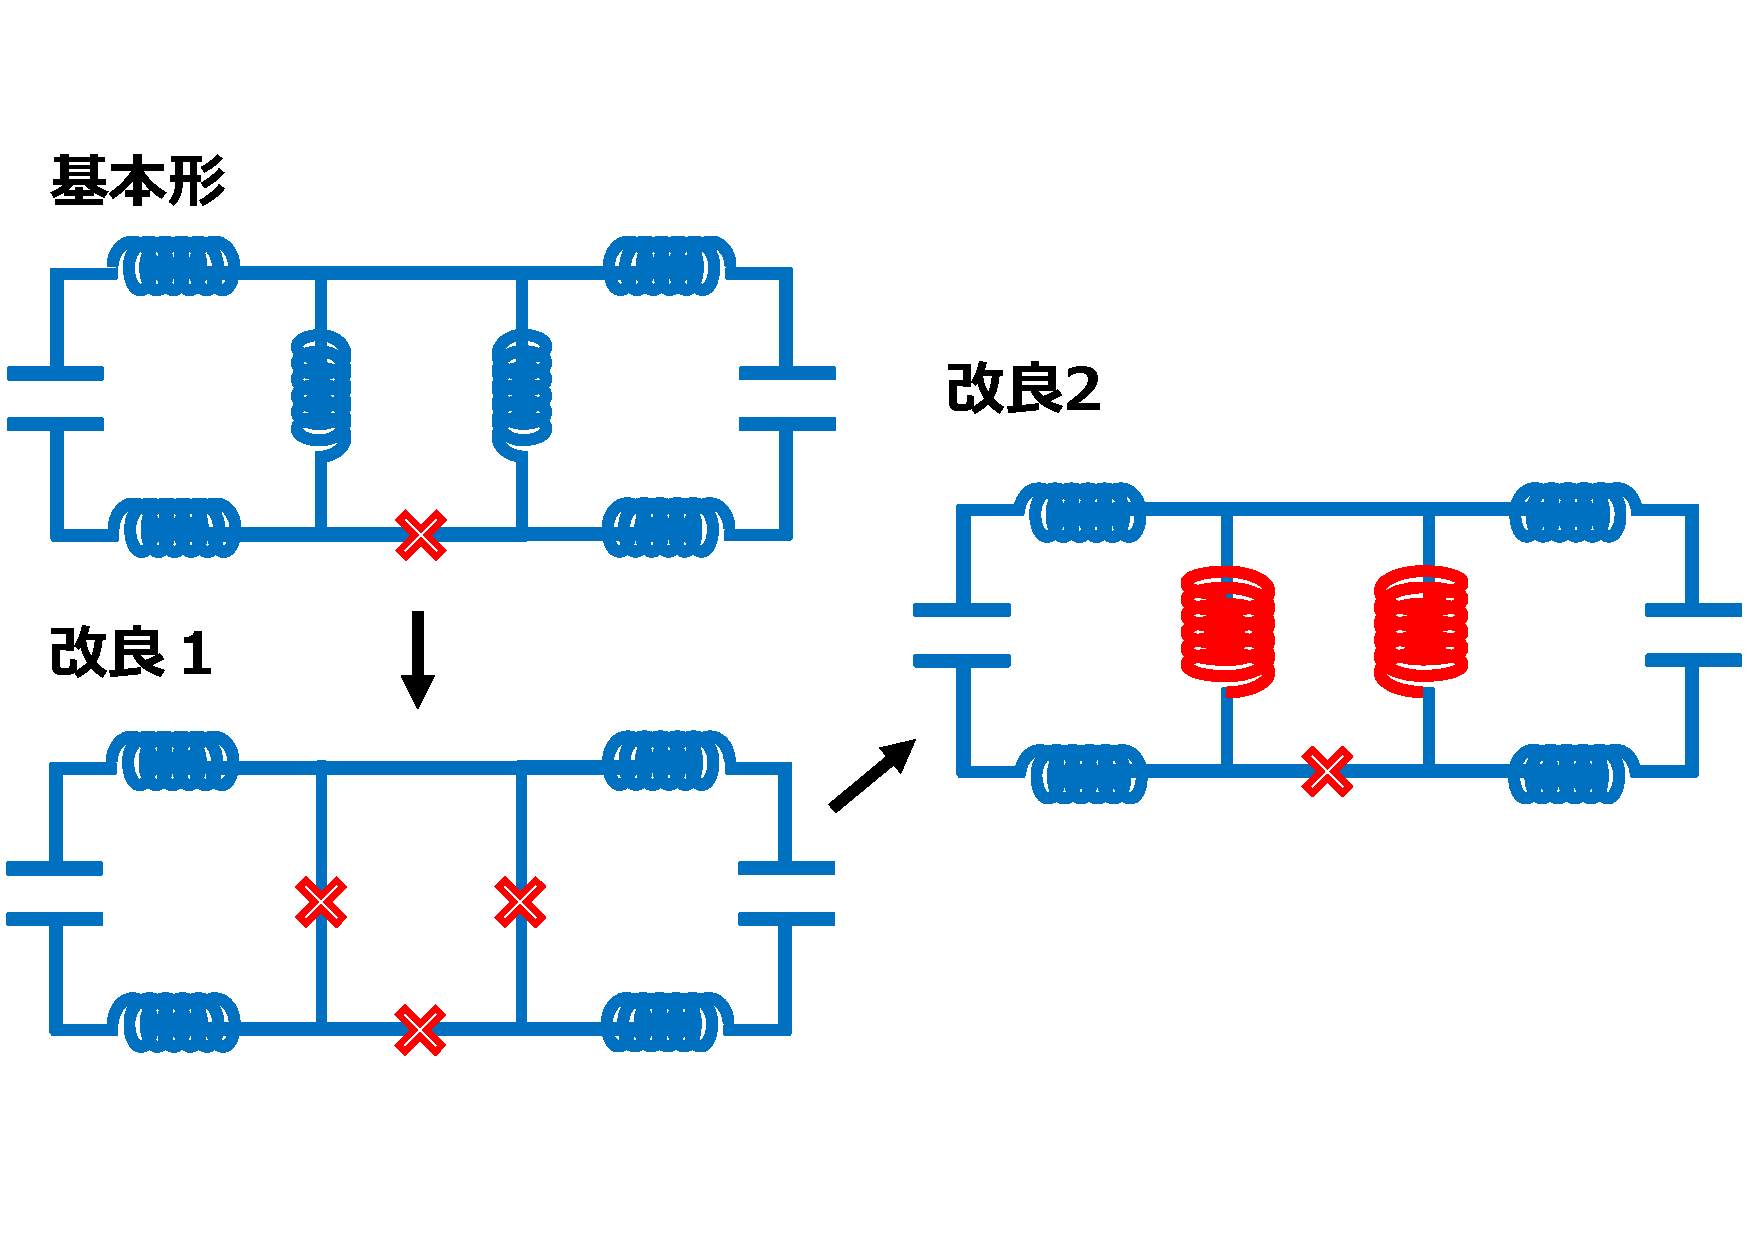
\includegraphics[width=14cm]{sample.pdf}
            \caption{サンプル図}
        \end{figure}
        上図は作成サンプルの回路図を模式的に表したものである。共振器とrf-SQUID間は線路に流れる電流により生じる磁場を介して結合している。模式図のように素子間が完全に接地した状態の結合のことをGalvanic結合と呼ぶ。この構造では、素子間の相互インダクタンスが接地部分の自己インダクタンスとほぼ等しくなるため非常に強力な相互インダクタンスを得ることができる。

        設計のポイントは①rf-SQUID-共振器間の相互インダクタンス増強と②rf-SQUIDスクリーニングパラメータの精密な製造である。この2つのパラメータは結合強度を向上する上で非常に重要な因子となる。
        この2つのパラメータが結合強度向上に大きく寄与するということを基本型であるrf-SQUIDの遷移スペクトルの計算を通して論拠する。
    \subsection{遷移スペクトル計算}
        基本型の回路のハミルトニアンは
        
        この結果は解析的に見積もることができる。計算過程はやや煩雑であるので補足に記載したので参照されたい。
        計算結果からわかるように結合モードの遷移周波数間のエネルギー差はそのまま基底変換する前の結合強度を示している。よって実験から結合強度を見積もるにはこのスペクトルを設計値を初期条件に設定した上で関数フィッティングを行う。得られたパラメータから結合強度を見積もる。
        設計の段階でもこのことを念頭に置いた上で設計する。
        各変数を順に固定した後で測定環境を含め最適な値を探した。
        それぞれのサンプルの測定時期であるが
    \subsection{メインループによる変調}
    \subsection{$\beta$ ループによる変調}

    \subsection{回路デザイン}

    \subsection{電磁界シミュレーション}
    

\section{製造}

    \subsection{製造パラメータ}

    \subsection{二重角度蒸着}

\section{測定サンプル}

    \subsection{回路パラメータ}
